\section{Software requirements document}{
	\subsection{Functional model}{
		\subsubsection{Use case diagram}{
			\begin{figure}[htbp]
				\begin{center}
					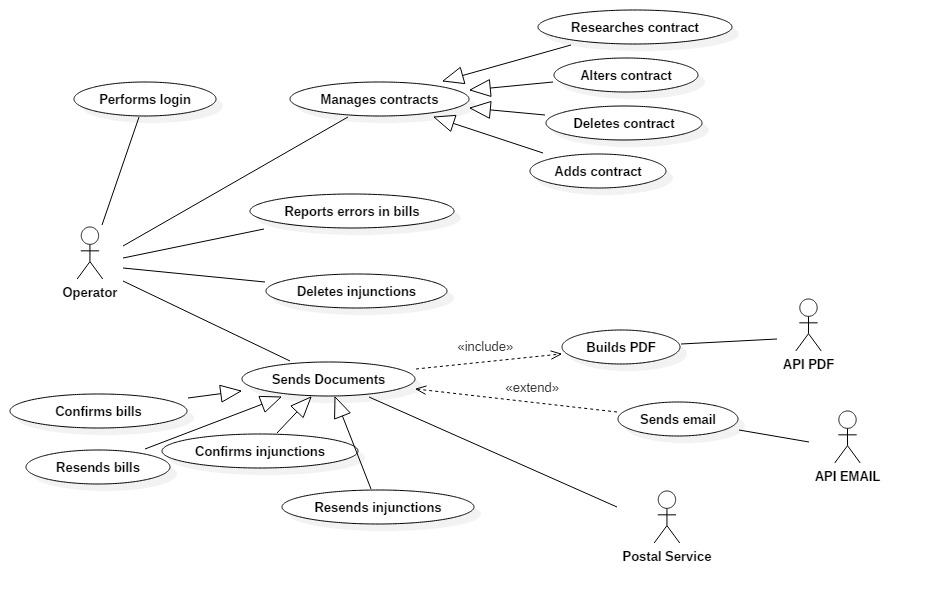
\includegraphics[width=15cm]{images/UseCaseDiagram.jpg}
				\end{center}
				\caption{Use case diagram}
			\end{figure}
		}
		\clearpage
		\subsubsection{Cockburn tables}{
			\begin{table}[ht]
			\begin{tabular}{|p{4cm}|p{10cm}|}
			\hline
				\centering \vspace{1mm} \bfseries{Use case} \vspace{1mm} & 
				\vspace{1mm} Performs login \vspace{1mm}\\
			\hline
				\centering \vspace{1mm} \bfseries{Goal in context} \vspace{1mm} & 
				\vspace{1mm} The operator wants to authenticate \vspace{1mm}\\
			\hline
				\centering \vspace{1mm} \bfseries{Preconditions} \vspace{1mm} & 
				\vspace{1mm} The goal is to let the operator log into the system inserting the right credentials \vspace{1mm}\\
			\hline
				\centering \vspace{1mm} \bfseries{Success end condition} \vspace{1mm} & 
				\vspace{1mm} The operator gets access to the system \vspace{1mm}\\
			\hline
				\centering \vspace{1mm} \bfseries{Failed end condition} \vspace{1mm} & 
				\vspace{1mm} The operator can't access to the system \vspace{1mm}\\
			\hline
				\centering \vspace{1mm} \bfseries{Primary actor} \vspace{1mm} & 
				\vspace{1mm} Operator \vspace{1mm}\\
			\hline
				\centering \vspace{1mm} \bfseries{Trigger} \vspace{1mm} & 
				\vspace{1mm} The operator starts the program \vspace{1mm}\\
			\hline
			\end{tabular}
			\end{table}

			\begin{table}[h]
			\begin{tabular}{|p{1cm}|p{6cm}|p{6cm}|}
			\hline
				\multicolumn{3}{|c|}{MAIN SCENARIO} \\
			\hline
				\centering \vspace{1mm} \bfseries{Step n.} \vspace{1mm} & \vspace{1mm} \bfseries{Operator} \vspace{1mm} & \vspace{1mm} \bfseries{System} \vspace{1mm}\\
			\hline
				\vspace{1mm} 1 \vspace{1mm} &
				\vspace{1mm} The operator starts the program \vspace{1mm} & 
				\vspace{1mm} \vspace{1mm} \\
			\hline
				\vspace{1mm} 2 \vspace{1mm} &
				\vspace{1mm} \vspace{1mm} & 
				\vspace{1mm} The system shows the "Login" mockup\vspace{1mm} \\
			\hline
				\vspace{1mm} 3 \vspace{1mm} &
				\vspace{1mm} The operator fills all field in the "Login" mockup \vspace{1mm} & 
				\vspace{1mm} \vspace{1mm} \\
			\hline
				\vspace{1mm} 4 \vspace{1mm} &
				\vspace{1mm} \vspace{1mm} & 
				\vspace{1mm} The system enables the "Login" button in the "Login" mockup \vspace{1mm} \\
			\hline
				\vspace{1mm} 5 \vspace{1mm} &
				\vspace{1mm} The operator presses the "Login" button in the "Login" mockup \vspace{1mm} & 
				\vspace{1mm} \vspace{1mm} \\
			\hline
				\vspace{1mm} 6 \vspace{1mm} &
				\vspace{1mm} \vspace{1mm} & 
				\vspace{1mm} The system shows the "Home" mockup\vspace{1mm} \\
			\hline
			\end{tabular}
			\end{table}
			\begin{table}[h]
			\begin{tabular}{|p{2cm}|p{6cm}|p{6cm}|}
			\hline
				\multicolumn{3}{|c|}{EXTENSION n.1} \\
			\hline
				\centering \vspace{1mm} \bfseries{Step n.} \vspace{1mm} & \vspace{1mm} \bfseries{Operator} \vspace{1mm} & \vspace{1mm} \bfseries{System} \vspace{1mm}\\
			\hline
				\vspace{1mm} 6.1 \vspace{1mm} &
				\vspace{1mm} \vspace{1mm} & 
				\vspace{1mm} The system shows the "Login - error" mockup\vspace{1mm} \\
			\hline
				\vspace{1mm} 7.1 \vspace{1mm} &
				\vspace{1mm} The operator presses the "ok" button in the "Login - error" mockup\vspace{1mm} & 
				\vspace{1mm} \vspace{1mm} \\
			\hline
				\vspace{1mm} 8.1 \vspace{1mm} &
				\vspace{1mm} \vspace{1mm} & 
				\vspace{1mm} Go to step 3 \vspace{1mm} \\
			\hline
			\end{tabular}
			\end{table}

			\clearpage

			\begin{table}[h]
			\begin{tabular}{|p{4cm}|p{10cm}|}
			\hline
				\centering \vspace{1mm} \bfseries{Use case} \vspace{1mm} & 
				\vspace{1mm} Researches contract \vspace{1mm}\\
			\hline
				\centering \vspace{1mm} \bfseries{Goal in context} \vspace{1mm} & 
				\vspace{1mm} The operator can be able to read information about the contract researched \vspace{1mm}\\
			\hline
				\centering \vspace{1mm} \bfseries{Preconditions} \vspace{1mm} & 
				\vspace{1mm} The operator must be logged in and he has compiled almost one field in the “Registry management” mockup \vspace{1mm}\\
			\hline
				\centering \vspace{1mm} \bfseries{Success end condition} \vspace{1mm} & 
				\vspace{1mm} The operator reads the informations about the contract researched \vspace{1mm}\\
			\hline
				\centering \vspace{1mm} \bfseries{Failed end condition} \vspace{1mm} & 
				\vspace{1mm} There aren’t contracts in the system \vspace{1mm}\\
			\hline
				\centering \vspace{1mm} \bfseries{Primary actor} \vspace{1mm} & 
				\vspace{1mm} Operator \vspace{1mm}\\
			\hline
				\centering \vspace{1mm} \bfseries{Trigger} \vspace{1mm} & 
				\vspace{1mm} The operator clicks on “Search” button in the ”Registry management” mockup \vspace{1mm}\\
			\hline
			\end{tabular}
			\end{table}
			\begin{table}[h]
			\begin{tabular}{|p{2cm}|p{6cm}|p{6cm}|}
			\hline
				\multicolumn{3}{|c|}{MAIN SCENARIO} \\
			\hline
				\centering \vspace{1mm} \bfseries{Step n.} \vspace{1mm} & \vspace{1mm} \bfseries{Operator} \vspace{1mm} & \vspace{1mm} \bfseries{System} \vspace{1mm}\\
			\hline
				\vspace{1mm} 1 \vspace{1mm} &
				\vspace{1mm} The operator clicks on “Search” button in “Registry management”  mockup \vspace{1mm} & 
				\vspace{1mm} \vspace{1mm} \\
			\hline
				\vspace{1mm} 2 \vspace{1mm} &
				\vspace{1mm} \vspace{1mm} & 
				\vspace{1mm} The system shows in the table the details of the contracts founded. \vspace{1mm} \\
			\hline
			\end{tabular}
			\end{table}
			\begin{table}[h]
			\begin{tabular}{|p{2cm}|p{6cm}|p{6cm}|}
			\hline
				\multicolumn{3}{|c|}{EXTENSION n.1} \\
			\hline
				\centering \vspace{1mm} \bfseries{Step n.} \vspace{1mm} & \vspace{1mm} \bfseries{Operator} \vspace{1mm} & \vspace{1mm} \bfseries{System} \vspace{1mm}\\
			\hline
				\vspace{1mm} 3.1 \vspace{1mm} &
				\vspace{1mm} \vspace{1mm} & 
				\vspace{1mm} The system shows the “Registry management – Error” mockup \vspace{1mm} \\
			\hline
				\vspace{1mm} 4.1 \vspace{1mm} &
				\vspace{1mm} The operator clicks on the “Ok” button in the “Registry management – Error” mockup \vspace{1mm} & 
				\vspace{1mm} \vspace{1mm} \\
			\hline
			\end{tabular}
			\end{table}
			\begin{table}[h]
			\begin{tabular}{|p{2cm}|p{6cm}|p{6cm}|}
			\hline
				\multicolumn{3}{|c|}{SUBVARIATION n.1} \\
			\hline
				\centering \vspace{1mm} \bfseries{Step n.} \vspace{1mm} & \vspace{1mm} \bfseries{Operator} \vspace{1mm} & \vspace{1mm} \bfseries{System} \vspace{1mm}\\
			\hline
				\vspace{1mm} 1.2 \vspace{1mm} &
				\vspace{1mm} The operator leaves all field blank \vspace{1mm} & 
				\vspace{1mm} \vspace{1mm} \\
			\hline
				\vspace{1mm} 2.2 \vspace{1mm} &
				\vspace{1mm} \vspace{1mm} & 
				\vspace{1mm} The system shows details of all contracts present in the system \vspace{1mm} \\
			\hline
			\end{tabular}
			\end{table}

			\clearpage

			\begin{table}[h]
			\begin{tabular}{|p{4cm}|p{10cm}|}
			\hline
				\centering \vspace{1mm} \bfseries{Use case} \vspace{1mm} & 
				\vspace{1mm} Alters contract \vspace{1mm}\\
			\hline
				\centering \vspace{1mm} \bfseries{Goal in context} \vspace{1mm} & 
				\vspace{1mm} Modify a pre-existing contract \vspace{1mm}\\
			\hline
				\centering \vspace{1mm} \bfseries{Preconditions} \vspace{1mm} & 
				\vspace{1mm} The operator must be logged in, he has searched a contract and he has selected it from the table in the "Registry management"  mockup \vspace{1mm}\\
			\hline
				\centering \vspace{1mm} \bfseries{Success end condition} \vspace{1mm} & 
				\vspace{1mm} The operator has modified a pre-existing contract \vspace{1mm}\\
			\hline
				\centering \vspace{1mm} \bfseries{Failed end condition} \vspace{1mm} & 
				\vspace{1mm} The operator fills the fields with invalid characters The operator cancels the operation and system shows the “Registry management” mockup \vspace{1mm}\\
			\hline
				\centering \vspace{1mm} \bfseries{Primary actor} \vspace{1mm} & 
				\vspace{1mm} Operator \vspace{1mm}\\
			\hline
				\centering \vspace{1mm} \bfseries{Trigger} \vspace{1mm} & 
				\vspace{1mm} The operator clicks on the "Alter holder" button in the “Registry management” mockup \vspace{1mm}\\
			\hline
			\end{tabular}
			\end{table}
			\begin{table}[h]
			\begin{tabular}{|p{2cm}|p{6cm}|p{6cm}|}
			\hline
				\multicolumn{3}{|c|}{MAIN SCENARIO} \\
			\hline
				\centering \vspace{1mm} \bfseries{Step n.} \vspace{1mm} & \vspace{1mm} \bfseries{Operator} \vspace{1mm} & \vspace{1mm} \bfseries{System} \vspace{1mm}\\
			\hline
				\vspace{1mm} 1 \vspace{1mm} &
				\vspace{1mm} The operator clicks on the "Alter holder" button in “Registry management” mockup \vspace{1mm} & 
				\vspace{1mm} \vspace{1mm} \\
			\hline
				\vspace{1mm} 2 \vspace{1mm} &
				\vspace{1mm} \vspace{1mm} & 
				\vspace{1mm} The system shows the “Alter holder” mockup \vspace{1mm} \\
			\hline
				\vspace{1mm} 3 \vspace{1mm} &
				\vspace{1mm} The operator edits one or more fields \vspace{1mm} & 
				\vspace{1mm} \vspace{1mm} \\
			\hline
				\vspace{1mm} 4 \vspace{1mm} &
				\vspace{1mm} \vspace{1mm} & 
				\vspace{1mm} The system enables the “Alter” button associated with the field edited\vspace{1mm} \\
			\hline
				\vspace{1mm} 5 \vspace{1mm} &
				\vspace{1mm} The operator clicks on the “Alter” button\vspace{1mm} & 
				\vspace{1mm} \vspace{1mm} \\
			\hline
				\vspace{1mm} 6 \vspace{1mm} &
				\vspace{1mm} \vspace{1mm} & 
				\vspace{1mm} The system shows  the “Alter holder – Success”  mockup\vspace{1mm} \\
			\hline
				\vspace{1mm} 7 \vspace{1mm} &
				\vspace{1mm} The operator clicks on the “Ok” button in the “Alter holder – Success”  mockup\vspace{1mm} & 
				\vspace{1mm} \vspace{1mm} \\
			\hline
			\end{tabular}
			\end{table}
			\begin{table}[h]
			\begin{tabular}{|p{2cm}|p{6cm}|p{6cm}|}
			\hline
				\multicolumn{3}{|c|}{EXTENSION n.1} \\
			\hline
				\centering \vspace{1mm} \bfseries{Step n.} \vspace{1mm} & \vspace{1mm} \bfseries{Operator} \vspace{1mm} & \vspace{1mm} \bfseries{System} \vspace{1mm}\\
			\hline
				\vspace{1mm} 6.1 \vspace{1mm} &
				\vspace{1mm} \vspace{1mm} & 
				\vspace{1mm} The system shows the “Alter holder – Error”  mockup with the reference to the form that contains the error \vspace{1mm} \\
			\hline
				\vspace{1mm} 7.1 \vspace{1mm} &
				\vspace{1mm} The operator clicks on the “Ok” button in the “Alter holder – Error”  mockup \vspace{1mm} & 
				\vspace{1mm} \vspace{1mm} \\
			\hline
				\vspace{1mm} 8.1 \vspace{1mm} &
				\vspace{1mm} \vspace{1mm} & 
				\vspace{1mm} Go to step 2\vspace{1mm} \\
			\hline
			\end{tabular}
			\end{table}
			\begin{table}[h]
			\begin{tabular}{|p{2cm}|p{6cm}|p{6cm}|}
			\hline
				\multicolumn{3}{|c|}{EXTENSION n.2} \\
			\hline
				\centering \vspace{1mm} \bfseries{Step n.} \vspace{1mm} & \vspace{1mm} \bfseries{Operator} \vspace{1mm} & \vspace{1mm} \bfseries{System} \vspace{1mm}\\
			\hline
				\vspace{1mm} 3.2 \vspace{1mm} &
				\vspace{1mm} The operator clicks on the “Back” button in the “Alter holder”  mockup \vspace{1mm} & 
				\vspace{1mm} \vspace{1mm} \\
			\hline
				\vspace{1mm} 4.2 \vspace{1mm} &
				\vspace{1mm} \vspace{1mm} & 
				\vspace{1mm} The system shows the “Registry management” mockup \vspace{1mm} \\
			\hline
			\end{tabular}
			\end{table}
			
			\clearpage

			\begin{table}[h]
			\begin{tabular}{|p{4cm}|p{10cm}|}
			\hline
				\centering \vspace{1mm} \bfseries{Use case} \vspace{1mm} & 
				\vspace{1mm} Deletes contract \vspace{1mm}\\
			\hline
				\centering \vspace{1mm} \bfseries{Goal in context} \vspace{1mm} & 
				\vspace{1mm}The operator wants to delete a contract  \vspace{1mm}\\
			\hline
				\centering \vspace{1mm} \bfseries{Preconditions} \vspace{1mm} & 
				\vspace{1mm}The operator must be logged in and he has selected a contract from the table described in mockup “Registry management” \vspace{1mm}\\
			\hline
				\centering \vspace{1mm} \bfseries{Success end condition} \vspace{1mm} & 
				\vspace{1mm}The operator deletes the selected contract \vspace{1mm}\\
			\hline
				\centering \vspace{1mm} \bfseries{Failed end condition} \vspace{1mm} & 
				\vspace{1mm} The operator can’t delete the selected contract 

				The operator cancels the operation\vspace{1mm}\\
			\hline
				\centering \vspace{1mm} \bfseries{Primary actor} \vspace{1mm} & 
				\vspace{1mm} Operator \vspace{1mm}\\
			\hline
				\centering \vspace{1mm} \bfseries{Trigger} \vspace{1mm} & 
				\vspace{1mm} The operator clicks on the “Delete” button in the “Registry management” mockup\vspace{1mm}\\
			\hline
			\end{tabular}
			\end{table}
			\begin{table}[h]
			\begin{tabular}{|p{2cm}|p{6cm}|p{6cm}|}
			\hline
				\multicolumn{3}{|c|}{MAIN SCENARIO} \\
			\hline
				\vspace{1mm} \bfseries{Step n.} \vspace{1mm} &
				\vspace{1mm} \bfseries{Operator} \vspace{1mm} & 
				\vspace{1mm} \bfseries{System} \vspace{1mm}\\
			\hline
				\vspace{1mm} 1 \vspace{1mm} &
				\vspace{1mm} The operator clicks on the “Delete”  button  in the “Registry management”  mockup \vspace{1mm} & 
				\vspace{1mm} \vspace{1mm} \\
			\hline
				\vspace{1mm} 2 \vspace{1mm} &
				\vspace{1mm} \vspace{1mm} & 
				\vspace{1mm} The system shows the “Delete contract”  mockup \vspace{1mm} \\
			\hline
				\vspace{1mm} 3 \vspace{1mm} &
				\vspace{1mm} The operator clicks on the “Yes”  button  in the “Delete contract”  mockup \vspace{1mm} & 
				\vspace{1mm} \vspace{1mm} \\
			\hline
				\vspace{1mm} 4 \vspace{1mm} &
				\vspace{1mm} \vspace{1mm} & 
				\vspace{1mm} The system shows the “Delete contract - Success”  mockup \vspace{1mm} \\
			\hline
				\vspace{1mm} 5 \vspace{1mm} &
				\vspace{1mm} The operator clicks on the “Ok”  button  in the “Delete contract - Success”  mockup\vspace{1mm} & 
				\vspace{1mm} \vspace{1mm} \\
			\hline
				\vspace{1mm} 6 \vspace{1mm} &
				\vspace{1mm} \vspace{1mm} & 
				\vspace{1mm} The system shows the mockup “Registry management” mockup \vspace{1mm} \\
			\hline	
			\end{tabular}
			\end{table}
			
			\begin{table}[h]
			\begin{tabular}{|p{2cm}|p{6cm}|p{6cm}|}
			\hline
				\multicolumn{3}{|c|}{EXTENSION n.1} \\
			\hline
				\vspace{1mm} \bfseries{Step n.} \vspace{1mm} & 
				\vspace{1mm} \bfseries{Operator} \vspace{1mm} & 
				\vspace{1mm} \bfseries{System} \vspace{1mm}\\
			\hline
				\vspace{1mm} 3.1 \vspace{1mm} &
				\vspace{1mm} \vspace{1mm} & 
				\vspace{1mm} The system shows the “Delete contract - Error" mockup \vspace{1mm} \\
			\hline
				\vspace{1mm} 4.1 \vspace{1mm} &
				\vspace{1mm} The operator clicks on the “Ok”  button  in the “ Delete contract - Error ”  mockup\vspace{1mm} & 
				\vspace{1mm} \vspace{1mm} \\
			\hline
				\vspace{1mm} 5.1 \vspace{1mm} &
				\vspace{1mm} \vspace{1mm} & 
				\vspace{1mm} Go to step 6 \vspace{1mm} \\
			\hline
			\end{tabular}
			\end{table}

			\begin{table}[h]
			\begin{tabular}{|p{2cm}|p{6cm}|p{6cm}|}
			\hline
				\multicolumn{3}{|c|}{EXTENSION n.2} \\
			\hline
				\vspace{1mm} \bfseries{Step n.} \vspace{1mm} & 
				\vspace{1mm} \bfseries{Operator} \vspace{1mm} & 
				\vspace{1mm} \bfseries{System} \vspace{1mm}\\
			\hline
				\vspace{1mm} 3.2 \vspace{1mm} &
				\vspace{1mm} The operator clicks on the “No”  button  in the “Delete contract”  mockup \vspace{1mm} & 
				\vspace{1mm} \vspace{1mm} \\
			\hline
				\vspace{1mm} 4.2 \vspace{1mm} &
				\vspace{1mm} \vspace{1mm} & 
				\vspace{1mm} Go to step 6 \vspace{1mm} \\
			\hline
			\end{tabular}
			\end{table}
			
			\clearpage

			\begin{table}[h]
			\begin{tabular}{|p{4cm}|p{10cm}|}
			\hline
				\centering \vspace{1mm} \bfseries{Use case} \vspace{1mm} & 
				\vspace{1mm} Reports errors in bills \vspace{1mm}\\
			\hline
				\centering \vspace{1mm} \bfseries{Goal in context} \vspace{1mm} & 
				\vspace{1mm} The operator wants to report errors in bills  \vspace{1mm}\\
			\hline
				\centering \vspace{1mm} \bfseries{Preconditions} \vspace{1mm} & 
				\vspace{1mm} The operator must be logged in and he has selected a bill in the bills’ table of the “Bills queue” mockup \vspace{1mm}\\
			\hline
				\centering \vspace{1mm} \bfseries{Success end condition} \vspace{1mm} & 
				\vspace{1mm} The operator reports and error in a bill \vspace{1mm}\\
			\hline
				\centering \vspace{1mm} \bfseries{Failed end condition} \vspace{1mm} & 
				\vspace{1mm} The operator clicks on the “Cancel” button \vspace{1mm}\\
			\hline
				\centering \vspace{1mm} \bfseries{Primary actor} \vspace{1mm} & 
				\vspace{1mm} Operator \vspace{1mm}\\
			\hline
				\centering \vspace{1mm} \bfseries{Trigger} \vspace{1mm} & 
				\vspace{1mm} The operator clicks on the “Report error” button in the “Bills”  mockup \vspace{1mm}\\
			\hline
			\end{tabular}
			\end{table}

			\begin{table}[h]
			\begin{tabular}{|p{2cm}|p{6cm}|p{6cm}|}
			\hline
				\multicolumn{3}{|c|}{MAIN SCENARIO} \\
			\hline
				\vspace{1mm} \bfseries{Step n.} \vspace{1mm} &
				\vspace{1mm} \bfseries{Operator} \vspace{1mm} & 
				\vspace{1mm} \bfseries{System} \vspace{1mm}\\
			\hline
				\vspace{1mm} 1 \vspace{1mm} &
				\vspace{1mm} The operator clicks on the “Report error” button in “Bills” mockup \vspace{1mm} & 
				\vspace{1mm} \vspace{1mm} \\
			\hline
				\vspace{1mm} 2 \vspace{1mm} &
				\vspace{1mm} \vspace{1mm} & 
				\vspace{1mm} The system shows the “Report error” mockup \vspace{1mm} \\
			\hline
				\vspace{1mm} 3 \vspace{1mm} &
				\vspace{1mm} The operator fills the “Report’s specifications” field in the “Report error”  mockup \vspace{1mm} & 
				\vspace{1mm} \vspace{1mm} \\
			\hline
				\vspace{1mm} 4 \vspace{1mm} &
				\vspace{1mm} \vspace{1mm} & 
				\vspace{1mm} The system enables the “Send” button \vspace{1mm} \\
			\hline
				\vspace{1mm} 5 \vspace{1mm} &
				\vspace{1mm} The operator clicks on the “Send” button \vspace{1mm} & 
				\vspace{1mm} \vspace{1mm} \\
			\hline
				\vspace{1mm} 6 \vspace{1mm} &
				\vspace{1mm} \vspace{1mm} & 
				\vspace{1mm} The system shows the “Send ” mockup \vspace{1mm} \\
			\hline	
			\end{tabular}
			\end{table}
			
			\begin{table}[h]
			\begin{tabular}{|p{2cm}|p{6cm}|p{6cm}|}
			\hline
				\multicolumn{3}{|c|}{EXTENSION n.1} \\
			\hline
				\centering \vspace{1mm} \bfseries{Step n.} \vspace{1mm} & \vspace{1mm} \bfseries{Operator} \vspace{1mm} & \vspace{1mm} \bfseries{System} \vspace{1mm}\\
			\hline
				\vspace{1mm} 3.1 \vspace{1mm} &
				\vspace{1mm} The operator clicks on the “Cancel” button \vspace{1mm} & 
				\vspace{1mm} \vspace{1mm} \\
			\hline
				\vspace{1mm} 4.1 \vspace{1mm} &
				\vspace{1mm} \vspace{1mm} & 
				\vspace{1mm} Go to step 8\vspace{1mm} \\
			\hline
			\end{tabular}
			\end{table}

			\begin{table}[h]
			\begin{tabular}{|p{2cm}|p{6cm}|p{6cm}|}
			\hline
				\multicolumn{3}{|c|}{EXTENSION n.2} \\
			\hline
				\centering \vspace{1mm} \bfseries{Step n.} \vspace{1mm} & \vspace{1mm} \bfseries{Operator} \vspace{1mm} & \vspace{1mm} \bfseries{System} \vspace{1mm}\\
			\hline
				\vspace{1mm} 5.2 \vspace{1mm} &
				\vspace{1mm} The operator clicks on the “Cancel” button\vspace{1mm} & 
				\vspace{1mm} \vspace{1mm} \\
			\hline
				\vspace{1mm} 6.2\vspace{1mm} &
				\vspace{1mm} \vspace{1mm} & 
				\vspace{1mm} Go to step 8\vspace{1mm} \\
			\hline
			\end{tabular}
			\end{table}

			\clearpage

			\begin{table}[h]
			\begin{tabular}{|p{4cm}|p{10cm}|}
			\hline
				\centering \vspace{1mm} \bfseries{Use case} \vspace{1mm} & 
				\vspace{1mm} Deletes injunction\vspace{1mm}\\
			\hline
				\centering \vspace{1mm} \bfseries{Goal in context} \vspace{1mm} & 
				\vspace{1mm} The operator wants to delete an injunction that has the “non-issued” state \vspace{1mm}\\
			\hline
				\centering \vspace{1mm} \bfseries{Preconditions} \vspace{1mm} & 
				\vspace{1mm} The operator must be logged in and has selected an injunction from the injunctions’ table in “Injunctions queue” mockup \vspace{1mm}\\
			\hline
				\centering \vspace{1mm} \bfseries{Success end condition} \vspace{1mm} & 
				\vspace{1mm} The operator deletes one or more injunctions from the injunctions’ table in “Injunctions queue” mockup \vspace{1mm}\\
			\hline
				\centering \vspace{1mm} \bfseries{Failed end condition} \vspace{1mm} & 
				\vspace{1mm} The operator doesn’t delete the injunction from the table\vspace{1mm}\\
			\hline
				\centering \vspace{1mm} \bfseries{Primary actor} \vspace{1mm} & 
				\vspace{1mm} Operator \vspace{1mm}\\
			\hline
				\centering \vspace{1mm} \bfseries{Trigger} \vspace{1mm} & 
				\vspace{1mm} The operator clicks on the “Delete” button in the “Injunctions queue” mockup\vspace{1mm}\\
			\hline
			\end{tabular}
			\end{table}

			\begin{table}[h]
			\begin{tabular}{|p{2cm}|p{6cm}|p{6cm}|}
			\hline
				\multicolumn{3}{|c|}{MAIN SCENARIO}\\
			\hline
				\centering \vspace{1mm} \bfseries{Step n.} \vspace{1mm} & \vspace{1mm} \bfseries{Operator} \vspace{1mm} & \vspace{1mm} \bfseries{System} \vspace{1mm}\\
			\hline
				\vspace{1mm} 1 \vspace{1mm} &
				\vspace{1mm} The operator clicks on the “Delete” button  in the “Injunctions queue” mockup\vspace{1mm} & 
				\vspace{1mm} \vspace{1mm} \\
			\hline
				\vspace{1mm} 2 \vspace{1mm} &
				\vspace{1mm} \vspace{1mm} & 
				\vspace{1mm} The system shows the “Delete Injunction - Success” mockup\vspace{1mm} \\
			\hline
				\vspace{1mm} 3 \vspace{1mm} &
				\vspace{1mm} The operator clicks on the “Ok”  button\vspace{1mm} & 
				\vspace{1mm} \vspace{1mm} \\
			\hline
				\vspace{1mm} 4 \vspace{1mm} &
				\vspace{1mm} \vspace{1mm} & 
				\vspace{1mm} The system shows the “Injunctions queue”  mockup\vspace{1mm} \\
			\hline
			\end{tabular}
			\end{table}
			
			\begin{table}[h]
			\begin{tabular}{|p{2cm}|p{6cm}|p{6cm}|}
			\hline
				\multicolumn{3}{|c|}{EXTENSION n.1}\\
			\hline
				\centering \vspace{1mm} \bfseries{Step n.} \vspace{1mm} & \vspace{1mm} \bfseries{Operator} \vspace{1mm} & \vspace{1mm} \bfseries{System} \vspace{1mm}\\
			\hline
				\vspace{1mm} 2.2\vspace{1mm} &
				\vspace{1mm} \vspace{1mm} & 
				\vspace{1mm} The system shows the “Delete Injunction – Error” mockup\vspace{1mm} \\
			\hline
				\vspace{1mm} 3.2\vspace{1mm} &
				\vspace{1mm} The operator clicks on the “Ok”  button\vspace{1mm} & 
				\vspace{1mm} \vspace{1mm} \\
			\hline
			\end{tabular}
			\end{table}
			
			\clearpage

			\begin{table}[h]
			\begin{tabular}{|p{4cm}|p{10cm}|}
			\hline
				\centering \vspace{1mm} \bfseries{Use case} \vspace{1mm} & 
				\vspace{1mm} Confirms bills\vspace{1mm}\\
			\hline
				\centering \vspace{1mm} \bfseries{Goal in context} \vspace{1mm} & 
				\vspace{1mm} The operator wants to confirm a single or a group of bills  \vspace{1mm}\\
			\hline
				\centering \vspace{1mm} \bfseries{Preconditions} \vspace{1mm} & 
				\vspace{1mm} The operator must be logged in and he has selected a bill/s in the bills’ table of the “Bills queue” mockup\vspace{1mm}\\
			\hline
				\centering \vspace{1mm} \bfseries{Success end condition} \vspace{1mm} & 
				\vspace{1mm} The operator confirms a bill\vspace{1mm}\\
			\hline
				\centering \vspace{1mm} \bfseries{Failed end condition} \vspace{1mm} & 
				\vspace{1mm} The operator cancels the operation\vspace{1mm}\\
			\hline
				\centering \vspace{1mm} \bfseries{Primary actor} \vspace{1mm} & 
				\vspace{1mm} Operator \vspace{1mm}\\
			\hline
				\centering \vspace{1mm} \bfseries{Trigger} \vspace{1mm} & 
				\vspace{1mm} The operator clicks on the “Confirm” button in the “Bills queue” mockup\vspace{1mm}\\
			\hline
			\end{tabular}
			\end{table}

			\begin{table}[h]
			\begin{tabular}{|p{2cm}|p{6cm}|p{6cm}|}
			\hline
				\multicolumn{3}{|c|}{MAIN SCENARIO}\\
			\hline
				\centering \vspace{1mm} \bfseries{Step n.} \vspace{1mm} & \vspace{1mm} \bfseries{Operator} \vspace{1mm} & \vspace{1mm} \bfseries{System} \vspace{1mm}\\
			\hline
				\vspace{1mm} 1 \vspace{1mm} &
				\vspace{1mm} The operator clicks on the “Confirm” button in the “Bills queue” mockup \vspace{1mm} & 
				\vspace{1mm} \vspace{1mm} \\
			\hline
				\vspace{1mm} 2 \vspace{1mm} &
				\vspace{1mm} \vspace{1mm} & 
				\vspace{1mm} The system shows the “Build PDF” mockup \vspace{1mm} \\
			\hline
				\vspace{1mm} 3 \vspace{1mm} &
				\vspace{1mm} The operator clicks on the “Send PDF” button in the “Build PDF” mockup \vspace{1mm} & 
				\vspace{1mm} \vspace{1mm} \\
			\hline
				\vspace{1mm} 4 \vspace{1mm} &
				\vspace{1mm} \vspace{1mm} & 
				\vspace{1mm} The system shows the “Send PDF” mockup \vspace{1mm} \\
			\hline
				\vspace{1mm} 5 \vspace{1mm} &
				\vspace{1mm} The operator clicks on the “Ok” button \vspace{1mm} & 
				\vspace{1mm} \vspace{1mm} \\
			\hline
				\vspace{1mm} 6 \vspace{1mm} &
				\vspace{1mm} \vspace{1mm} & 
				\vspace{1mm} The system shows the “Bills queue” mockup\vspace{1mm} \\
			\hline
			\end{tabular}
			\end{table}
			
			\begin{table}[h]
			\begin{tabular}{|p{2cm}|p{6cm}|p{6cm}|}
			\hline
				\multicolumn{3}{|c|}{EXTENSION n.1}\\
			\hline
				\centering \vspace{1mm} \bfseries{Step n.} \vspace{1mm} & \vspace{1mm} \bfseries{Operator} \vspace{1mm} & \vspace{1mm} \bfseries{System} \vspace{1mm}\\
			\hline
				\vspace{1mm} 3.1 \vspace{1mm} &
				\vspace{1mm} The operator clicks on the “Cancels” button in the “Build PDF” mockup \vspace{1mm} & 
				\vspace{1mm} \vspace{1mm} \\
			\hline
				\vspace{1mm} 4.1 \vspace{1mm} &
				\vspace{1mm} \vspace{1mm} & 
				\vspace{1mm} Go to step 6\vspace{1mm} \\
			\hline
			\end{tabular}
			\end{table}
			\begin{table}[h]
			\begin{tabular}{|p{2cm}|p{6cm}|p{6cm}|}
			\hline
				\multicolumn{3}{|c|}{EXTENSION n.2}\\
			\hline
				\centering \vspace{1mm} \bfseries{Step n.} \vspace{1mm} & \vspace{1mm} \bfseries{Operator} \vspace{1mm} & \vspace{1mm} \bfseries{System} \vspace{1mm}\\
			\hline
				\vspace{1mm} 4.2 \vspace{1mm} &
				\vspace{1mm} \vspace{1mm} & 
				\vspace{1mm} The system shows the “Send PDF” mockup in which the field “Log address’ Error” is visible\vspace{1mm} \\
			\hline
				\vspace{1mm} 5.2 \vspace{1mm} &
				\vspace{1mm} Go to step 5\vspace{1mm} & 
				\vspace{1mm} \vspace{1mm} \\
			\hline
			\end{tabular}
			\end{table}
			\begin{table}[h]
			\begin{tabular}{|p{2cm}|p{6cm}|p{6cm}|}
			\hline
				\multicolumn{3}{|c|}{SUBVARIATION n.1}\\
			\hline
				\centering \vspace{1mm} \bfseries{Step n.} \vspace{1mm} & \vspace{1mm} \bfseries{Operator} \vspace{1mm} & \vspace{1mm} \bfseries{System} \vspace{1mm}\\
			\hline
				\vspace{1mm} 1.3\vspace{1mm} &
				\vspace{1mm} The operator clicks on the “Confirm” button in the “Bills queue” mockup after he has selected multiple rows from the table or has clicked on the “Select All” button\vspace{1mm} & 
				\vspace{1mm} \vspace{1mm} \\
			\hline
				\vspace{1mm} 2.3\vspace{1mm} &
				\vspace{1mm} \vspace{1mm} & 
				\vspace{1mm} The system shows the “Build PDF - Multiple” mockup \vspace{1mm} \\
			\hline
				\vspace{1mm} 3.3\vspace{1mm} &
				\vspace{1mm} The operator clicks on the “Send PDFs” button in the “Build PDF - Multiple” mockup \vspace{1mm} & 
				\vspace{1mm} \vspace{1mm} \\
			\hline
				\vspace{1mm} 4.3\vspace{1mm} &
				\vspace{1mm} \vspace{1mm} & 
				\vspace{1mm} The system shows the “Send PDF - Multiple” mockup\vspace{1mm} \\
			\hline
				\vspace{1mm} 5.3\vspace{1mm} &
				\vspace{1mm} Go to step 5\vspace{1mm} & 
				\vspace{1mm} \vspace{1mm} \\
			\hline
			\end{tabular}
			\end{table}
			
			\clearpage
	
			\begin{table}[h]
			\begin{tabular}{|p{4cm}|p{10cm}|}
			\hline
				\centering \vspace{1mm} \bfseries{Use case} \vspace{1mm} & 
				\vspace{1mm} Resends bills\vspace{1mm}\\
			\hline
				\centering \vspace{1mm} \bfseries{Goal in context} \vspace{1mm} & 
				\vspace{1mm}The operator wants to resend a bill that has the “Issued” state \vspace{1mm}\\
			\hline
				\centering \vspace{1mm} \bfseries{Preconditions} \vspace{1mm} & 
				\vspace{1mm} The operator must be logged in and he has selected a bill in the bills’ table of the “Bills” mockup\vspace{1mm}\\
			\hline
				\centering \vspace{1mm} \bfseries{Success end condition} \vspace{1mm} & 
				\vspace{1mm}The operator must be logged in and he has selected a bill in the bills’ table of the “Bills” mockup \vspace{1mm}\\
			\hline
				\centering \vspace{1mm} \bfseries{Failed end condition} \vspace{1mm} & 
				\vspace{1mm}The operator cancels the operation The PDF interface is not available \vspace{1mm}\\
			\hline
				\centering \vspace{1mm} \bfseries{Primary actor} \vspace{1mm} & 
				\vspace{1mm} Operator \vspace{1mm}\\
			\hline
				\centering \vspace{1mm} \bfseries{Trigger} \vspace{1mm} & 
				\vspace{1mm} The operator clicks on “Build PDF” button in the “Bills” mockup \vspace{1mm}\\
			\hline
			\end{tabular}
			\end{table}

			\begin{table}[h]
			\begin{tabular}{|p{2cm}|p{6cm}|p{6cm}|}
			\hline
				\multicolumn{3}{|c|}{MAIN SCENARIO}\\
			\hline
				\centering \vspace{1mm} \bfseries{Step n.} \vspace{1mm} & \vspace{1mm} \bfseries{Operator} \vspace{1mm} & \vspace{1mm} \bfseries{System} \vspace{1mm}\\
			\hline
				\vspace{1mm} 1 \vspace{1mm} &
				\vspace{1mm} The operator clicks on the “Build PDF” button in the “Bills” mockup\vspace{1mm} & 
				\vspace{1mm} \vspace{1mm} \\
			\hline
				\vspace{1mm} 2 \vspace{1mm} &
				\vspace{1mm} \vspace{1mm} & 
				\vspace{1mm} The system shows the “Build PDF” mockup\vspace{1mm} \\
			\hline
				\vspace{1mm} 3\vspace{1mm} &
				\vspace{1mm} The operator clicks on the “Send PDF” button in the “Build PDF” mockup\vspace{1mm} & 
				\vspace{1mm} \vspace{1mm} \\
			\hline
				\vspace{1mm} 4\vspace{1mm} &
				\vspace{1mm} \vspace{1mm} & 
				\vspace{1mm} The system shows the “Send PDF” mockup\vspace{1mm} \\
			\hline
				\vspace{1mm} 5\vspace{1mm} &
				\vspace{1mm} The operator clicks on the “Ok” button\vspace{1mm} & 
				\vspace{1mm} \vspace{1mm} \\
			\hline
				\vspace{1mm} 6\vspace{1mm} &
				\vspace{1mm} \vspace{1mm} & 
				\vspace{1mm} The system shows the “Registry management” mockup\vspace{1mm} \\
			\hline
			\end{tabular}
			\end{table}
			
			\begin{table}[h]
			\begin{tabular}{|p{2cm}|p{6cm}|p{6cm}|}
			\hline
				\multicolumn{3}{|c|}{EXTENSION n.1}\\
			\hline
				\centering \vspace{1mm} \bfseries{Step n.} \vspace{1mm} & \vspace{1mm} \bfseries{Operator} \vspace{1mm} & \vspace{1mm} \bfseries{System} \vspace{1mm}\\
			\hline
				\vspace{1mm} 3.1\vspace{1mm} &
				\vspace{1mm} The operator clicks on the “Cancel” button in the “Build PDF” mockup \vspace{1mm} & 
				\vspace{1mm} \vspace{1mm} \\
			\hline
				\vspace{1mm} 4.1\vspace{1mm} &
				\vspace{1mm} \vspace{1mm} & 
				\vspace{1mm} The system shows the “Bills” mockup\vspace{1mm} \\
			\hline
			\end{tabular}
			\end{table}
			\begin{table}[h]
			\begin{tabular}{|p{2cm}|p{6cm}|p{6cm}|}
			\hline
				\multicolumn{3}{|c|}{EXTENSION n.2}\\
			\hline
				\centering \vspace{1mm} \bfseries{Step n.} \vspace{1mm} & \vspace{1mm} \bfseries{Operator} \vspace{1mm} & \vspace{1mm} \bfseries{System} \vspace{1mm}\\
			\hline
				\vspace{1mm} 4.2\vspace{1mm} &
				\vspace{1mm} \vspace{1mm} & 
				\vspace{1mm} The system shows the “Send PDF” mockup in which the “Log address’ error” form is visible \vspace{1mm} \\
			\hline
				\vspace{1mm} 5.2\vspace{1mm} &
				\vspace{1mm} Go to step 5\vspace{1mm} & 
				\vspace{1mm} \vspace{1mm} \\
			\hline
			\end{tabular}
			\end{table}
			\begin{table}[h]
			\begin{tabular}{|p{2cm}|p{6cm}|p{6cm}|}
			\hline
				\multicolumn{3}{|c|}{EXTENSION n.3}\\
			\hline
				\centering \vspace{1mm} \bfseries{Step n.} \vspace{1mm} & \vspace{1mm} \bfseries{Operator} \vspace{1mm} & \vspace{1mm} \bfseries{System} \vspace{1mm}\\
			\hline
				\vspace{1mm} 2.3\vspace{1mm} &
				\vspace{1mm} \vspace{1mm} & 
				\vspace{1mm} The system shows the “Build PDF – Error” mockup\vspace{1mm} \\
			\hline
				\vspace{1mm} 3.3\vspace{1mm} &
				\vspace{1mm} The operator clicks on the “Ok” button in the “Build PDF – Error” mockup\vspace{1mm} & 
				\vspace{1mm} \vspace{1mm} \\
			\hline
				\vspace{1mm} 4.3\vspace{1mm} &
				\vspace{1mm} Go to step 6\vspace{1mm} & 
				\vspace{1mm} \vspace{1mm} \\
			\hline
			\end{tabular}
			\end{table}
			
			\clearpage
	
			\begin{table}[h]
			\begin{tabular}{|p{4cm}|p{10cm}|}
			\hline
				\centering \vspace{1mm} \bfseries{Use case} \vspace{1mm} & 
				\vspace{1mm} Confirms injunctions\vspace{1mm}\\
			\hline
				\centering \vspace{1mm} \bfseries{Goal in context} \vspace{1mm} & 
				\vspace{1mm} The operator wants to send the injuction to the customer \vspace{1mm}\\
			\hline
				\centering \vspace{1mm} \bfseries{Preconditions} \vspace{1mm} & 
				\vspace{1mm} The operator must be logged in and he has selected an injunction from the table described in “Injunctions queue” mockup\vspace{1mm}\\
			\hline
				\centering \vspace{1mm} \bfseries{Success end condition} \vspace{1mm} & 
				\vspace{1mm} The system creates and sends the PDF\vspace{1mm}\\
			\hline
				\centering \vspace{1mm} \bfseries{Failed end condition} \vspace{1mm} & 
				\vspace{1mm} The operator cancels the operation 

				The PDF interface is not available \vspace{1mm}\\
			\hline
				\centering \vspace{1mm} \bfseries{Primary actor} \vspace{1mm} & 
				\vspace{1mm} Operator \vspace{1mm}\\
			\hline
				\centering \vspace{1mm} \bfseries{Trigger} \vspace{1mm} & 
				\vspace{1mm} The operator clicks on the “Confirm” button in “Injunctions queue” mockup \vspace{1mm}\\
			\hline
			\end{tabular}
			\end{table}

			\begin{table}[h]
			\begin{tabular}{|p{2cm}|p{6cm}|p{6cm}|}
			\hline
				\multicolumn{3}{|c|}{MAIN SCENARIO}\\
			\hline
				\centering \vspace{1mm} \bfseries{Step n.} \vspace{1mm} & \vspace{1mm} \bfseries{Operator} \vspace{1mm} & \vspace{1mm} \bfseries{System} \vspace{1mm}\\
			\hline
				\vspace{1mm} 1\vspace{1mm} &
				\vspace{1mm} The operator clicks on the “Confirm” button in “Injunctions queue” mockup\vspace{1mm} & 
				\vspace{1mm} \vspace{1mm} \\
			\hline
				\vspace{1mm} 2\vspace{1mm} &
				\vspace{1mm} \vspace{1mm} & 
				\vspace{1mm} The system shows the “Build PDF” mockup\vspace{1mm} \\
			\hline
				\vspace{1mm} 3\vspace{1mm} &
				\vspace{1mm} The operator clicks on the “Send PDF” button in “Build PDF” mockup\vspace{1mm} & 
				\vspace{1mm} \vspace{1mm} \\
			\hline
				\vspace{1mm} 4\vspace{1mm} &
				\vspace{1mm} \vspace{1mm} & 
				\vspace{1mm} The system shows the “Send PDF” mockup\vspace{1mm} \\
			\hline
				\vspace{1mm} 5\vspace{1mm} &
				\vspace{1mm} The operator clicks on the “Ok” button in the “Send PDF” mockup\vspace{1mm} & 
				\vspace{1mm} \vspace{1mm} \\
			\hline
				\vspace{1mm} 6\vspace{1mm} &
				\vspace{1mm} \vspace{1mm} & 
				\vspace{1mm} The system shows the “Registry management” mockup\vspace{1mm} \\
			\hline
			\end{tabular}
			\end{table}
			
			\begin{table}[h]
			\begin{tabular}{|p{2cm}|p{6cm}|p{6cm}|}
			\hline
				\multicolumn{3}{|c|}{EXTENSION n.1}\\
			\hline
				\centering \vspace{1mm} \bfseries{Step n.} \vspace{1mm} & \vspace{1mm} \bfseries{Operator} \vspace{1mm} & \vspace{1mm} \bfseries{System} \vspace{1mm}\\
			\hline
				\vspace{1mm} 3.1\vspace{1mm} &
				\vspace{1mm} The operator clicks on the “Cancel" button in "Build PDF" mockup\vspace{1mm} & 
				\vspace{1mm} \vspace{1mm} \\
			\hline
				\vspace{1mm} 4.1\vspace{1mm} &
				\vspace{1mm} \vspace{1mm} & 
				\vspace{1mm} The system shows the “Injunctions queue” mockup\vspace{1mm} \\
			\hline
			\end{tabular}
			\end{table}
			\begin{table}[h]
			\begin{tabular}{|p{2cm}|p{6cm}|p{6cm}|}
			\hline
				\multicolumn{3}{|c|}{EXTENSION n.2}\\
			\hline
				\centering \vspace{1mm} \bfseries{Step n.} \vspace{1mm} & \vspace{1mm} \bfseries{Operator} \vspace{1mm} & \vspace{1mm} \bfseries{System} \vspace{1mm}\\
			\hline
				\vspace{1mm} 4.2\vspace{1mm} &
				\vspace{1mm} \vspace{1mm} & 
				\vspace{1mm} The system shows the “Send PDF” mockup in which the “Log address’ error” form is visible \vspace{1mm} \\
			\hline
				\vspace{1mm} 5.2\vspace{1mm} &
				\vspace{1mm} Go to step 5\vspace{1mm} & 
				\vspace{1mm} \vspace{1mm} \\
			\hline
			\end{tabular}
			\end{table}
			\begin{table}[h]
			\begin{tabular}{|p{2cm}|p{6cm}|p{6cm}|}
			\hline
				\multicolumn{3}{|c|}{EXTENSION n.3}\\
			\hline
				\centering \vspace{1mm} \bfseries{Step n.} \vspace{1mm} & \vspace{1mm} \bfseries{Operator} \vspace{1mm} & \vspace{1mm} \bfseries{System} \vspace{1mm}\\
			\hline
				\vspace{1mm} 2.3\vspace{1mm} &
				\vspace{1mm} \vspace{1mm} & 
				\vspace{1mm} The system shows the “Build PDF – Error” mockup\vspace{1mm} \\
			\hline
				\vspace{1mm} 3.3\vspace{1mm} &
				\vspace{1mm} The operator clicks on the “Ok” button in the “Build PDF – Error” mockup\vspace{1mm} & 
				\vspace{1mm} \vspace{1mm} \\
			\hline
				\vspace{1mm} 4.3\vspace{1mm} &
				\vspace{1mm} \vspace{1mm} & 
				\vspace{1mm} Go to step 6\vspace{1mm} \\
			\hline
			\end{tabular}
			\end{table}
			
			\clearpage
	
			\begin{table}[h]
			\begin{tabular}{|p{4cm}|p{10cm}|}
			\hline
				\centering \vspace{1mm} \bfseries{Use case} \vspace{1mm} & 
				\vspace{1mm} Resends injunctions \vspace{1mm}\\
			\hline
				\centering \vspace{1mm} \bfseries{Goal in context} \vspace{1mm} & 
				\vspace{1mm} The operator wants to resend an injunction that has the “Issued” state \vspace{1mm}\\
			\hline
				\centering \vspace{1mm} \bfseries{Preconditions} \vspace{1mm} & 
				\vspace{1mm} The operator must be logged in and he has selected an injunction in the injunctions’ table of the “Injunctions” mockup \vspace{1mm}\\
			\hline
				\centering \vspace{1mm} \bfseries{Success end condition} \vspace{1mm} & 
				\vspace{1mm} The operator resends an injunction that has the “Issued” state	 \vspace{1mm}\\
			\hline
				\centering \vspace{1mm} \bfseries{Failed end condition} \vspace{1mm} & 
				\vspace{1mm} The operator cancels the operation \vspace{1mm}\\
			\hline
				\centering \vspace{1mm} \bfseries{Primary actor} \vspace{1mm} & 
				\vspace{1mm} Operator \vspace{1mm}\\
			\hline
				\centering \vspace{1mm} \bfseries{Trigger} \vspace{1mm} & 
				\vspace{1mm}The operator clicks on the “Build PDF” button in “Injunctions” mockup \vspace{1mm}\\
			\hline
			\end{tabular}
			\end{table}

			\begin{table}[h]
			\begin{tabular}{|p{2cm}|p{6cm}|p{6cm}|}
			\hline
				\multicolumn{3}{|c|}{MAIN SCENARIO}\\
			\hline
				\centering \vspace{1mm} \bfseries{Step n.} \vspace{1mm} & \vspace{1mm} \bfseries{Operator} \vspace{1mm} & \vspace{1mm} \bfseries{System} \vspace{1mm}\\
			\hline
				\vspace{1mm} 1\vspace{1mm} &
				\vspace{1mm} The operator clicks on the “Build PDF” button in “Injunctions” mockup \vspace{1mm} & 
				\vspace{1mm} \vspace{1mm} \\
			\hline
				\vspace{1mm} 2\vspace{1mm} &
				\vspace{1mm} \vspace{1mm} & 
				\vspace{1mm} The system shows the “Build PDF” mockup\vspace{1mm} \\
			\hline
				\vspace{1mm} 3\vspace{1mm} &
				\vspace{1mm} The operator clicks on the “Send PDF” button in the “Build PDF” mockup \vspace{1mm} & 
				\vspace{1mm} \vspace{1mm} \\
			\hline
				\vspace{1mm} 4\vspace{1mm} &
				\vspace{1mm} \vspace{1mm} & 
				\vspace{1mm} The system shows the “Send PDF” mockup \vspace{1mm} \\
			\hline
				\vspace{1mm} 5\vspace{1mm} &
				\vspace{1mm} The operator clicks on the “Ok” button in the “Send PDF” mockup \vspace{1mm} & 
				\vspace{1mm} \vspace{1mm} \\
			\hline
				\vspace{1mm} 6\vspace{1mm} &
				\vspace{1mm} \vspace{1mm} & 
				\vspace{1mm} The system shows the “Registry management” mockup\vspace{1mm} \\
			\hline
			\end{tabular}
			\end{table}
			
			\begin{table}[h]
			\begin{tabular}{|p{2cm}|p{6cm}|p{6cm}|}
			\hline
				\multicolumn{3}{|c|}{EXTENSION n.1}\\
			\hline
				\centering \vspace{1mm} \bfseries{Step n.} \vspace{1mm} & \vspace{1mm} \bfseries{Operator} \vspace{1mm} & \vspace{1mm} \bfseries{System} \vspace{1mm}\\
			\hline
				\vspace{1mm} 3.1\vspace{1mm} &
				\vspace{1mm} The operator clicks on the “Cancel” button in “Build PDF” mockup \vspace{1mm} & 
				\vspace{1mm} \vspace{1mm} \\
			\hline
				\vspace{1mm} 4.1\vspace{1mm} &
				\vspace{1mm} \vspace{1mm} & 
				\vspace{1mm} The system shows the “Injunctions” mockup\vspace{1mm} \\
			\hline
			\end{tabular}
			\end{table}
			\begin{table}[h]
			\begin{tabular}{|p{2cm}|p{6cm}|p{6cm}|}
			\hline
				\multicolumn{3}{|c|}{EXTENSION n.2}\\
			\hline
				\centering \vspace{1mm} \bfseries{Step n.} \vspace{1mm} & \vspace{1mm} \bfseries{Operator} \vspace{1mm} & \vspace{1mm} \bfseries{System} \vspace{1mm}\\
			\hline
				\vspace{1mm} 4.2 \vspace{1mm} &
				\vspace{1mm} \vspace{1mm} & 
				\vspace{1mm} The system shows the “Send PDF” mockup in which the “Log address’ error” form is visible  \vspace{1mm} \\
			\hline
				\vspace{1mm} 5.2\vspace{1mm} &
				\vspace{1mm} Go to step 5\vspace{1mm} & 
				\vspace{1mm} \vspace{1mm} \\
			\hline
			\end{tabular}
			\end{table}
			\begin{table}[h]
			\begin{tabular}{|p{2cm}|p{6cm}|p{6cm}|}
			\hline
				\multicolumn{3}{|c|}{EXTENSION n.3}\\
			\hline
				\centering \vspace{1mm} \bfseries{Step n.} \vspace{1mm} & \vspace{1mm} \bfseries{Operator} \vspace{1mm} & \vspace{1mm} \bfseries{System} \vspace{1mm}\\
			\hline
				\vspace{1mm} 2.3\vspace{1mm} &
				\vspace{1mm} \vspace{1mm} & 
				\vspace{1mm} The system shows the “Build PDF – Error” mockup\vspace{1mm} \\
			\hline
				\vspace{1mm} 3.3\vspace{1mm} &
				\vspace{1mm} The operator clicks on the “Ok” button in the “Build PDF – Error” mockup\vspace{1mm} & 
				\vspace{1mm} \vspace{1mm} \\
			\hline
				\vspace{1mm} 4.3\vspace{1mm} &
				\vspace{1mm} \vspace{1mm} & 
				\vspace{1mm} Go to step 6\vspace{1mm} \\
			\hline
			\end{tabular}
			\end{table}
			
						\begin{table}[h]
			\begin{tabular}{|p{4cm}|p{10cm}|}
			\hline
				\centering \vspace{1mm} \bfseries{Use case} \vspace{1mm} & 
				\vspace{1mm} Adds contract \vspace{1mm}\\
			\hline
				\centering \vspace{1mm} \bfseries{Goal in context} \vspace{1mm} & 
				\vspace{1mm} Create a new contract \vspace{1mm}\\
			\hline
				\centering \vspace{1mm} \bfseries{Preconditions} \vspace{1mm} & 
				\vspace{1mm} The operator must be logged in and clicks on the “Registry management” button from the “Home” mockup \vspace{1mm}\\
			\hline
				\centering \vspace{1mm} \bfseries{Success end condition} \vspace{1mm} & 
				\vspace{1mm} The operator adds a new contract \vspace{1mm}\\
			\hline
				\centering \vspace{1mm} \bfseries{Failed end condition} \vspace{1mm} & 
				\vspace{1mm} The operator doesn’t fill all fields - The operator cancels the operation \vspace{1mm}\\
			\hline
				\centering \vspace{1mm} \bfseries{Primary actor} \vspace{1mm} & 
				\vspace{1mm} Operator \vspace{1mm}\\
			\hline
				\centering \vspace{1mm} \bfseries{Trigger} \vspace{1mm} & 
				\vspace{1mm} The operator clicks on the “Add” button in the “Registry management” mockup \vspace{1mm}\\
			\hline
			\end{tabular}
			\end{table}

			\begin{table}[h]
			\begin{tabular}{|p{2cm}|p{6cm}|p{6cm}|}
			\hline
				\multicolumn{3}{|c|}{MAIN SCENARIO}\\
			\hline
				\centering \vspace{1mm} \bfseries{Step n.} \vspace{1mm} & \vspace{1mm} \bfseries{Operator} \vspace{1mm} & 
				\vspace{1mm} \bfseries{System} \vspace{1mm}\\
			\hline
				\vspace{1mm} 1 \vspace{1mm} &
				\vspace{1mm} The operator clicks on the “Add” button in the “Registry management” mockup \vspace{1mm} & 
				\vspace{1mm} \vspace{1mm} \\
			\hline
				\vspace{1mm} 2 \vspace{1mm} &
				\vspace{1mm} \vspace{1mm} & 
				\vspace{1mm} The system shows the “Add holder” mockup \vspace{1mm} \\
			\hline
				\vspace{1mm} 3 \vspace{1mm} &
				\vspace{1mm} The operator fills all fields and clicks on the “Add” button in the “Add holder” mockup \vspace{1mm} & 
				\vspace{1mm} \vspace{1mm} \\
			\hline
				\vspace{1mm} 4 \vspace{1mm} &
				\vspace{1mm} \vspace{1mm} & 
				\vspace{1mm} The system shows the “Add holder – Success”  mockup \vspace{1mm} \\
			\hline
				\vspace{1mm} 5 \vspace{1mm} &
				\vspace{1mm} The operator clicks on the “Ok” button in the “Add holder – Success”  mockup \vspace{1mm} & 
				\vspace{1mm} \vspace{1mm} \\
			\hline
				\vspace{1mm} 6 \vspace{1mm} &
				\vspace{1mm} \vspace{1mm} & 
				\vspace{1mm} The system shows the “Add holder”  mockup \vspace{1mm} \\
			\hline
			\end{tabular}
			\end{table}
			
			\begin{table}[h]
			\begin{tabular}{|p{2cm}|p{6cm}|p{6cm}|}
			\hline
				\multicolumn{3}{|c|}{EXTENSION n.1}\\
			\hline
				\centering \vspace{1mm} \bfseries{Step n.} \vspace{1mm} & \vspace{1mm} \bfseries{Operator} \vspace{1mm} & \vspace{1mm} \bfseries{System} \vspace{1mm}\\
			\hline
				\vspace{1mm} 4.1 \vspace{1mm} &
				\vspace{1mm} \vspace{1mm} & 
				\vspace{1mm} The system shows the “Add holder – Error”  mockup with reference to the field that contains the error \vspace{1mm} \\
			\hline
				\vspace{1mm} 5.1\vspace{1mm} &
				\vspace{1mm} The operator clicks on the “Ok” button in the “Add holder – Error”  mockup \vspace{1mm} & 
				\vspace{1mm} \vspace{1mm} \\
			\hline
				\vspace{1mm} 6.1\vspace{1mm} &
				\vspace{1mm} \vspace{1mm} & 
				\vspace{1mm} Go to step 2\vspace{1mm} \\
			\hline
			\end{tabular}
			\end{table}
			
			\begin{table}[h]
			\begin{tabular}{|p{2cm}|p{6cm}|p{6cm}|}
			\hline
				\multicolumn{3}{|c|}{EXTENSION n.2}\\
			\hline
				\centering \vspace{1mm} \bfseries{Step n.} \vspace{1mm} & \vspace{1mm} \bfseries{Operator} \vspace{1mm} & \vspace{1mm} \bfseries{System} \vspace{1mm}\\
			\hline
				\vspace{1mm} 3.2 \vspace{1mm} &
				\vspace{1mm} The operator clicks on the “Back” button in the “Add holder”  mockup \vspace{1mm} & 
				\vspace{1mm} \vspace{1mm} \\
			\hline
				\vspace{1mm} 4.2 \vspace{1mm} &
				\vspace{1mm} \vspace{1mm} & 
				\vspace{1mm} The system shows the “Registry management” mockup \vspace{1mm} \\
			\hline
			\end{tabular}
			\end{table}
			
			\clearpage
		}			
	}
}